
% JDR: At (my) normal speed, this takes less than 50 minutes.

\titleframe{Section 1.8}{Introduction to Linear Transformations}

\usetikzlibrary{datavisualization.formats.functions}
\usetikzlibrary{decorations.pathreplacing}


%%%%%%%%%%%%%%%%%%%%%%%%%%%%%%%%%%%%%%%%%%%%%%%%%%%%%%%%%%%%%%%%%%%

\begin{frame}
\frametitle{Motivation}

Let $A$ be an $m\times n$ matrix.  
\pause
For the matrix equation $Ax=b$ we have
learned to describe 
\begin{itemize}
\pause
\item the solution set: all $x$ in $\R^n$ making the equation true.
\pause
\item the column span: the set of all $b$ in $\R^m$ making the equation
  consistent.
\end{itemize}

\pause\bigskip
It turns out these two sets are very closely related to each other.
\note{Rank-nullity}

\pause\bigskip
In order to understand this relationship, it helps to think of the matrix $A$ as
a \emph{transformation} from $\R^n$ to $\R^m$.

\pause\bigskip
It's a special kind of transformation called a \emph{linear transformation}.

\pause\bigskip
This is also a way to understand the \emph{geometry} of \emph{matrices}.

\end{frame}


%%%%%%%%%%%%%%%%%%%%%%%%%%%%%%%%%%%%%%%%%%%%%%%%%%%%%%%%%%%%%%%%%%%

\begin{frame}
\frametitle{Transformations}

\vskip-3mm
\begin{defn}
  A \textbf{transformation} (or \textbf{function} or \textbf{map}) from $\R^n$
  to $\R^m$ is a rule $T$ that assigns to each vector $x$ in $\R^n$ a vector
  $T(x)$ in $\R^m$.
  \begin{itemize}
  \item<2-> $\R^n$ is called the \textbf{domain} of $T$ (the inputs).
  \item<3-> $\R^m$ is called the \textbf{codomain} of $T$ (the outputs).
  \item<4-> For $x$ in $\R^n$, the vector $T(x)$ in $\R^m$ is the \textbf{image} of
    $x$ under $T$.\\  \alert{Notation:} $x\mapsto T(x)$.
  \item<5-> The set of all images $\{T(x)\mid x\text{ in }\R^n\}$ is the
    \textbf{range} of $T$.
  \end{itemize}
  \begin{uncoverenv}<6->
  \alert{Notation:}\abovedisplayskip=2pt\abovedisplayshortskip=2pt
  \[ T\colon \R^n\To\R^m\sptxt{means}
  \text{$T$ is a transformation from $\R^n$ to $\R^m$.} \]
  \end{uncoverenv}
\end{defn}

\vskip -3mm
\hfill
\begin{tikzpicture}[scale=0.35, baseline, thin border nodes]
  \path[use as bounding box] (-3,-5.5) -- (15,3);
  \draw<2->[grid lines, light gray] (-3,-3) grid (3,3);

  \node<2-> (A) at (0,-4) {$\R^n$};
  \node<3-> (B) at (12,-4) {$\R^m$};
  \node<2-> at (0,-5) {domain};
  \node<3-> at (12,-5) {codomain};
  \draw<6->[->] (A.east) +(5mm,0) -- node[midway,above=1mm] {$T$}
    ($(B.west)-(5mm,0)$);

  \point<4->["$x$" left] (P) at (1,1,5);
%  \node<4->[point, label=left:$x$] (P) at (1,1.5) {};

  \begin{scope}[myxyz, xshift=12cm]
    \path[clip, resetxy] (-3,-3) rectangle (3,3);

    \def\v{(2,-1,1)}
    \def\w{(1,0,-1)}
  
    \node[coordinate] (X) at \v {};
    \node[coordinate] (Y) at \w {};

    \draw<3->[very thin] (-2,0,0) -- (0,0,0);
    \draw<3->[very thin] (0,-2,0) -- (0,0,0);
    \draw<3->[very thin] (0,0,-2) -- (0,0,0);

    \begin{scope}[x=(X), y=(Y), transformxy]
      \fill<5->[seq4!10, nearly opaque] (-1,-1) rectangle (1,1);
      \draw<5->[step=.5cm, seq4!30, very thin] (-1,-1) grid (1,1);
      \point<4->["$T(x)$" {font=\tiny,fill=none,below}] (Q) at (-.5,.5);
      \node<5->[coordinate,
          pin={[pin edge={very thin,-},pin distance=3mm,anchor=north]-70:range}]
        at (0.1,1) {};
    \end{scope}

    \draw<3->[->, very thin] (0,0,0) -- (2,0,0);
    \draw<3->[->, very thin] (0,0,0) -- (0,2,0);
    \draw<3->[->, very thin] (0,0,0) -- (0,0,2);

    \draw<3->[resetxy] (-3,-3) rectangle (3,3);

  \end{scope}

  \pic<7->[scale=.4, "$T$"] (machine) at (6,0) {machine};
  \node[coordinate] (IN) at (6cm-24pt/.35,0) {};
  \node[coordinate] (OUT) at (6cm+24pt/.35,0) {};
  \draw<7->[->, shorten >=.35mm, shorten <=.35mm] (P.east)
    .. controls +(0:1cm) and +(180:1cm) .. (IN);
  \draw<7->[->, shorten >=.35mm, shorten <=.35mm] (OUT)
    .. controls +(0:1cm) and +(190:2cm) .. (Q.west);

  \draw<4-6| handout:0>[|->, shorten >=.35mm, shorten <=.35mm] 
    (P.east) .. controls +(0:5cm) and +(190:5cm) .. (Q.west);

\end{tikzpicture}
\hfill
\begin{uncoverenv}<7->
\begin{minipage}[c]{.35\textwidth}
  It may help to think of $T$ as a ``machine'' that takes $x$ as an input, and
  gives you $T(x)$ as the output.
\end{minipage}
\end{uncoverenv}
\hfill\null


\end{frame}


%%%%%%%%%%%%%%%%%%%%%%%%%%%%%%%%%%%%%%%%%%%%%%%%%%%%%%%%%%%%%%%%%%%

\begin{frame}
\frametitle{Functions from Calculus}

Many of the functions you know and love have domain and codomain $\R$.
\pause
\abovedisplayskip=2mm\abovedisplayshortskip=2mm\belowdisplayskip=2mm
\[ \sin\colon\R\To\R \qquad \sin(x) =
  \left(\,\parbox{.5\textwidth}{
    the length of the opposite edge over the hypotenuse of a right
    triangle with angle $x$ in radians}\,\right) \]
\pause
Note how I've written down the \emph{rule} that defines the function $\sin$.
\pause
\[ f\colon\R\To\R \qquad f(x) = x^2 \]
\pause
Note that ``$x^2$'' is sloppy (but common) notation for a function: it doesn't
have a name!

\pause\bigskip
You may be used to thinking of a function in terms of its graph.
\medskip

\hfill
\begin{tikzpicture}[baseline]
  \datavisualization[school book axes,
      all axes={ticks=none},
      visualize as smooth line/.list={sin},
      sin={style=seq1}]

    data[format=function, set=sin] {
      var x : interval[-2:2] ;
      func y = sin(\value x r);
    };

  %\node[point, label=below:$x$] at (1,0) {};
  \point["$x$" below] at (1,0);
  %\node[point, label={[label distance=1.2mm]above:$(x,\sin x)$}] at (1,{sin(1 r)}) {};
  \point["${(x,\sin x)}$" {label distance=1.2mm, above}] at (1,{sin(1 r)});
\end{tikzpicture}
\hfill
\begin{minipage}[c]{.5\textwidth}\raggedright
  \pause
  The horizontal axis is the domain, and the vertical axis is the codomain.

  \pause\medskip
  This is fine when the domain and codomain are $\R$, but it's hard to do when
  they're $\R^2$ and $\R^3$!
  \pause
  You need
  \only<-9| handout:0>{\underline{\phantom{five}}}%
  \only<10->{five}
  dimensions to draw that graph.

\end{minipage}
\hfill\null

\end{frame}


%%%%%%%%%%%%%%%%%%%%%%%%%%%%%%%%%%%%%%%%%%%%%%%%%%%%%%%%%%%%%%%%%%%

\begin{frame}
\frametitle{Matrix Transformations}

Most of the transformations we encounter in this class will come from (surprise)
matrices!

\pause
\begin{defn}
  Let $A$ be an $m\times n$ matrix.  The \textbf{matrix transformation}
  associated to $A$ is the transformation
  \[ T\colon \R^n \To \R^m \sptxt{defined by} T(x) = Ax. \]
  \pause
  In other words, $T$ takes the vector $x$ in $\R^n$ to the vector $Ax$ in
  $\R^m$. 
\end{defn}

\pause
\begin{itemize}
\item \namedbox{top}{\strut}The \emph{domain} of $T$ is \pause $\R^n$, which is
  the number of
  \blankuntil{6}{\emph{columns\/}}
  of $A$.
\pause\pause
\item The \emph{codomain} of $T$ is \pause $\R^m$, which is the number of
  \blankuntil{9}{\emph{rows\/}} of $A$.
\pause\pause
\item The \emph{range} of $T$ is the set of all images of $T$:
  \[ T(x) = Ax = 
  \mat{| |, , |; v_1 v_2 \cdots, v_n; | |, , |}\vec{x_1 x_2 \vdots, x_n}
  = x_1v_1 + x_2v_2 + \cdots + x_nv_n. \]
  \namedbox{bottom}{\strut}This is the
  \pause 
  \emph{column span\/} of $A$.  It is a span of vectors in the codomain.
\end{itemize}
\pause
\begin{tikzpicture}[remember picture, overlay]
  \draw[decoration={brace, amplitude=2mm}, decorate, thick, red] 
    let \p1=($(current page.north west) + (1.2cm,0)$) in
      (\p1 |- bottom.south) -- 
        node[above=2mm, midway, sloped, text width=5cm, align=center] 
        {Your life will be much easier if you just remember these.}
      (\p1 |- top.north);
\end{tikzpicture}

\end{frame}


%%%%%%%%%%%%%%%%%%%%%%%%%%%%%%%%%%%%%%%%%%%%%%%%%%%%%%%%%%%%%%%%%%%

\begin{frame}
\frametitle{Matrix Transformations}
\framesubtitle{Example}

\def\A{\mat{1 1; 0 1; 1 1}}
Let $A = \A$ and let $T(x) = Ax$, so
$T\colon\R^{\blankuntil{2}{2}}\to\R^{\blankuntil{3}{3}}$.

\pause[4]%
\begin{itemize}
\item
  $\text{If } u = \vec{3 4} \sptxt{then}
  T(u) = \webonlycmd{\A\vec{3 4} = \vec{7 4 7}.}$

\pause
\item
  Let $b = \vec{7 5 7}$.  Find $v$ in $\R^{\blankuntil{6}{2}}$ such that
  $T(v) = b$.
  \pause[7]%
  Is there more than one?

  \begin{webonly}\smallskip
  We want to find $v$ such that $T(v) = Av = b$.  We know how to do that:
  \[ \A v = \vec{7 5 7}
    \longsquiggly[\parbox{\widthof{\small augmented}}
      {\small\centering augmented matrix}]
      \amat{1 1 7; 0 1 5; 1 1 7}
    \longsquiggly[\parbox{\widthof{\small reduce}}
      {\small\centering row reduce}]
    \amat{1 0 2; 0 1 5; 0 0 0}. \]
  This gives $x = 2$ and $y = 5$, or $v = \vec{2 5}$ (unique).  
  In other words,
  \[ T(v) = \A\vec{2 5} = \vec{7 5 7}. \]
  \end{webonly}

\end{itemize}

\end{frame}


%%%%%%%%%%%%%%%%%%%%%%%%%%%%%%%%%%%%%%%%%%%%%%%%%%%%%%%%%%%%%%%%%%%

\begin{frame}
\frametitle{Matrix Transformations}
\framesubtitle{Example, continued}

\def\A{\mat{1 1; 0 1; 1 1}}
Let $A = \A$ and let $T(x) = Ax$, so $T\colon\R^2\to\R^3$.

\begin{itemize}
\pause
\item Is there any $c$ in $\R^3$ such that there is more than one $v$ in $\R^2$ with
  $T(v) = c$? 

  \pause\smallskip
  \alert{Translation:} is there any $c$ in $\R^3$ such that the solution set of
  $Ax = c$ has more than one vector $v$ in it?

  \pause\smallskip
  The solution set of $Ax = c$ is a translate of the solution set of
  $Ax = b$ (from before), which has \blankuntil{5}{one} vector in it.
  \pause[6]%
  So the solution set to $Ax = c$ has only one vector.
  \pause
  So no!

  \pause\medskip
\item Find $c$ such that there is \emph{no} $v$ with $T(v) = c$.

  \pause\smallskip
  \alert{Translation:} Find $c$ such that $Ax = c$ is inconsistent.

  \pause\smallskip
  \alert{Translation:} Find $c$ not in the column span of $A$ (i.e., the range
    of $T$).
    \pause
    We could draw a picture, or notice:
    $a\vec{1 0 1} + b\vec{1 1 1} = \vec{a+b b a+b}$.
    \pause
    So anything in the column span has the same first and last coordinate.
    \pause
    So $c = \Bigl(\smallveciii123\Bigr)$ is not in the column span (for example).

\end{itemize}

\end{frame}


%%%%%%%%%%%%%%%%%%%%%%%%%%%%%%%%%%%%%%%%%%%%%%%%%%%%%%%%%%%%%%%%%%%

\begin{frame}
\frametitle{Matrix Transformations}
\framesubtitle{Geometric example}

Let $A = \mat{1 0 0; 0 1 0; 0 0 0}$ and let $T(x) = Ax$, so
$T\colon\R^{\blankuntil{2}{3}}\to\R^{\blankuntil{2}{3}}$.  
\pause[3]
Then
\[ T\vec{x y z} = \mat{1 0 0; 0 1 0; 0 0 0}\vec{x y z} = \vec{x y 0}. \]
\pause
This is
\pause
\emph{projection onto the $xy$-axis}.  Picture:

\begin{center}
\begin{tikzpicture}[myxyz, scale=0.5]
  \path[clip, resetxy] (-7,-4) rectangle (7,4);

  \begin{scope}[arrows={|[width=2pt]->[width=2pt]}, shorten=2pt]
    \draw (-1,-1,-2.5) node[point, seq2] {}
      -- (-1,-1,0);
    \draw (-2,2,-1) node[point, seq5] {}
      -- (-2,2,0);
  \end{scope}

  \begin{scope}[transformxy]
    \fill[white, nearly opaque] (-3, -3) rectangle (3, 3);
    \draw[step=1cm, help lines] (-3, -3) grid (3, 3);
  \end{scope}

  \begin{scope}[arrows={|[width=2pt]->[width=2pt]}, shorten=2pt]
    \draw (1,2,3) node[point,seq1] {}
      -- (1,2,0) node[point,seq1] {};
    \point[seq2] at (-1,-1,0);
    \point[seq5] at (-2,2,0);
    \draw (2,-1,2) node[point,seq3] {}
      -- (2,-1,0) node[point,seq3] {};
    \draw (0,-2,1) node[point,seq4] {}
      -- (0,-2,0) node[point,seq4] {};
  \end{scope}

\end{tikzpicture}
\end{center}

\end{frame}


%%%%%%%%%%%%%%%%%%%%%%%%%%%%%%%%%%%%%%%%%%%%%%%%%%%%%%%%%%%%%%%%%%%

\begin{frame}
\frametitle{Matrix Transformations}
\framesubtitle{Geometric example}

Let $A = \mat{-1 0; 0 1}$ and let $T(x) = Ax$, so
$T\colon\R^{\blankuntil{2}{2}}\to\R^{\blankuntil{2}{2}}$.  
\pause[3]
Then
\[ T\vec{x y} = \mat{-1 0; 0 1}\vec{x y} = \vec{-x y}. \]
\pause
This is
\pause
\emph{reflection over the $y$-axis}.  Picture:

\def\theo{
\includegraphics[width=4cm]{figures/theo2.jpg}}

\vfill
\hbox to \linewidth{\hss
\begin{tikzpicture}
  \node (theo1) at (0,0,0) {\theo};
  \draw[->,opacity=.3] (-1.8,0) -- (1.8,0);
  \draw[->,opacity=.3] (0,-1.8) -- (0,1.8);

  \begin{scope}[xshift=7cm]
  \node[xscale=-1] (theo2) at (0,0,0) {\theo};
  \draw[->,opacity=.3] (-1.8,0) -- (1.8,0);
  \draw[->,opacity=.3] (0,-1.8) -- (0,1.8);
  \end{scope}

  \draw[->] (theo1.20)
    to[out=20,in=160] node[midway,above] {$T$} (theo2.20);
\end{tikzpicture}
\hss}
\vfill

\end{frame}


%%%%%%%%%%%%%%%%%%%%%%%%%%%%%%%%%%%%%%%%%%%%%%%%%%%%%%%%%%%%%%%%%%%

\def\sheep{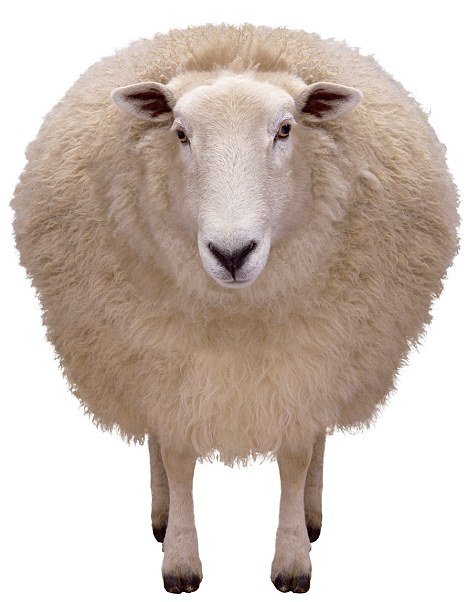
\includegraphics[width=2cm]{figures/sheep.jpg}}

\begin{pollframe}

Let $A = \mat{1 1; 0 1}$ and let $T(x) = Ax$, so $T\colon\R^2\to\R^2$.
($T$ is called a \textbf{shear}.)

\begin{poll}
\medskip
\begin{bluebox}[Poll]{.8\textwidth}
  What does $T$ do to this sheep?\\[1mm]
  \alert{Hint:} first draw a picture what it does to
  the box \emph{around} the sheep.
\end{bluebox}


\vfill
\hbox to \linewidth{\hss
\begin{tikzpicture}[axes/.pic={
    \draw[->,opacity=.5] (-.8,0) -- (.8,0);
    \draw[->,opacity=.5] (0,-.8) -- (0,.8);
  }]

  \node (sheep1) {\sheep} pic {axes};

 \path (4,0) node[rotate=90] (sheep2) {\sheep} pic {axes};
 \path (7,0) node[cm={1,0,1,1,(0,0)}] (sheep3) {\sheep} pic {axes};
 \path (9.8,0) node (sheep4) {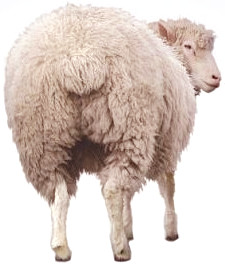
\includegraphics[width=2cm]{figures/sheep_back.jpg}} pic {axes};

  \draw[->,very thick,yshift=1cm] (sheep1.20)
    to[out=20, in=160, "$T$"] (sheep2.north |- sheep1.20);

  \path (4,1.4) node[seq-blue] {$A$}
      ++(3,0) node[seq-blue] {$B$}
      ++(2.8,0) node[seq-blue] {$C$};

  \useasboundingbox (0,-2.1);

  \draw<2->[dashed,seq-blue] (5.4,-1.4) rectangle (8.7,1.7);
  \node<2->[seq-blue] (SS) at (5,-2) {sheared sheep};
  \draw<2->[seq-blue,->,shorten=2pt] (SS.east) to[out=0,in=-90] (7,-1.4);

\end{tikzpicture}
\hss}
\vfill
\end{poll}

\end{pollframe}


%%%%%%%%%%%%%%%%%%%%%%%%%%%%%%%%%%%%%%%%%%%%%%%%%%%%%%%%%%%%%%%%%%%

\begin{frame}
\frametitle{Linear Transformations}

\displayskips{3pt}
\alert{Recall:} If $A$ is a matrix, $u,v$ are vectors, and $c$ is a scalar, then
\[ A(u+v) = Au + Av \qquad A(cv) = cAv. \]
\pause
So if $T(x) = Ax$ is a matrix transformation then,
\textcolor<4->{blue}{
\[ T(u+v) = T(u) + T(v)  \qquad  T(cv) = cT(v). \]}%
\pause
This property is so special that it has its own name.

\pause\smallskip
\begin{defn}
  A transformation $T\colon\R^n\to\R^m$ is \textbf{linear} if it satisfies the
  above \textcolor{blue}{equations} for all vectors $u,v$ in $\R^n$ and all
  scalars $c$.
\end{defn}

\pause
In other words, $T$ ``respects'' addition and scalar multiplication.

\pause\bigskip
\alert{Check:} if $T$ is linear, then
\[ T(0) = 0 \qquad T(cu + dv) = cT(u) + dT(v) \]
for all vectors $u,v$ and scalars $c,d$.
\pause
More generally,
\[ T\bigl( c_1v_1 + c_2v_2 + \cdots + c_nv_n \bigr)
 = c_1 T(v_1) + c_2 T(v_2) + \cdots + c_n T(v_n). \]
\pause
In engineering this is called \textbf{superposition}.

\end{frame}


%%%%%%%%%%%%%%%%%%%%%%%%%%%%%%%%%%%%%%%%%%%%%%%%%%%%%%%%%%%%%%%%%%%

\begin{frame}
\frametitle{Linear Transformations}
\framesubtitle{Dilation}

Define $T\colon\R^2\to\R^2$ by $T(x) = 1.5x$.  Is $T$ linear?  Check:
\pause
\[\begin{split} 
  T(u+v) &= \webonlycmd{1.5(u+v) = 1.5u + 1.5v = T(u) + T(v)} \\
  T(cv) &= \webonlycmd{1.5(cv) = c(1.5v) = c(Tv).} \end{split} \]
\pause
So $T$ satisfies the two equations, hence $T$ is linear.

\pause\medskip
This is called \textbf{dilation} or \textbf{scaling} (by a factor of $1.5$).
Picture:

\pause

\def\theo{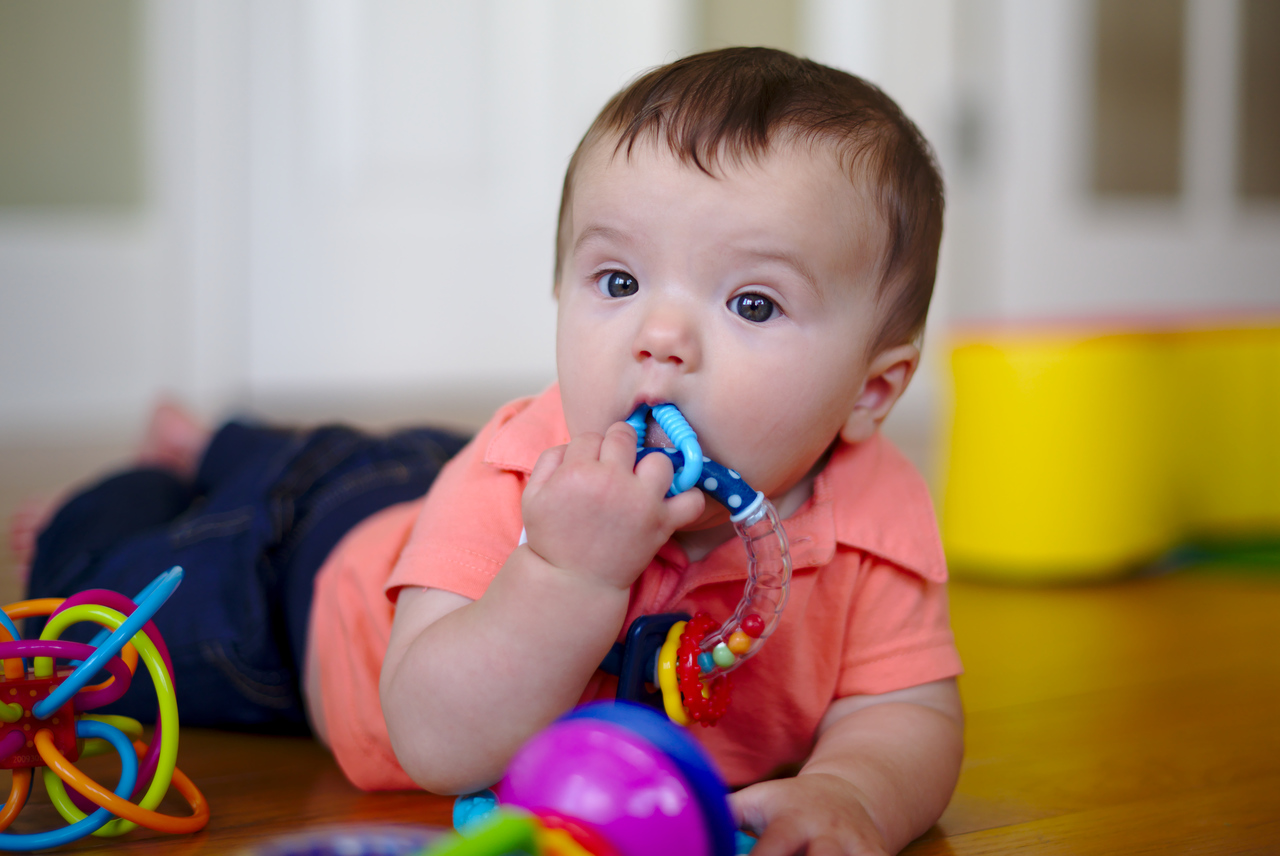
\includegraphics[width=3.5cm]{figures/theo3.jpg}}

\vfill
\hbox to \linewidth{\hss
\begin{tikzpicture}
  \node (theo1) at (0,0,0) {\theo};
  \draw[->,opacity=.6] (-1.3,0) -- (1.3,0);
  \draw[->,opacity=.6] (0,-1.3) -- (0,1.3);

  \begin{scope}[xshift=7cm]
  \node[scale=1.5] (theo2) at (0,0,0) {\theo};
  \draw[->,opacity=.6] (-1.3,0) -- (1.3,0);
  \draw[->,opacity=.6] (0,-1.3) -- (0,1.3);
  \end{scope}

  \draw[->] ($(theo1.east)+(0,.3)$)
    to[bend left, "$T$"] ($(theo2.west)+(0,.3)$);
\end{tikzpicture}
\hss}
\vfill

\end{frame}


%%%%%%%%%%%%%%%%%%%%%%%%%%%%%%%%%%%%%%%%%%%%%%%%%%%%%%%%%%%%%%%%%%%

\def\arcarrow#1;{
  \pgfmathanglebetweenpoints{\pgfpoint{0cm}{0cm}}{\pgfpointanchor{#1}{center}}
  \let\sangle=\pgfmathresult
  \draw[|->, shorten=1mm] 
    let \p1 = (#1.center), \n1={veclen(\x1,\y1)} in
      (#1) arc[radius=\n1, delta angle=90, start angle=\sangle];
}

\begin{frame}
\frametitle{Linear Transformations}
\framesubtitle{Rotation}

Define $T\colon\R^2\to\R^2$ by
\[ T\vec{x y} = \vec{-y x}. \]
Is $T$ linear?  Check:
\pause
\[\begin{split} 
  T\left(\vec{u_1 u_2} + \vec{v_1 v_2}\right)
    &= \webonlycmd{\vec{-u_2 u_1} + \vec{-v_2 v_1}
         = \vec{-(u_2+v_2) (u_1+v_1)} = T\vec{u_1+u_2 v_1+v_2}} \\
  T\left(c\vec{v_1 v_2}\right)
  &= \webonlycmd{T\vec{cv_1 cv_2} = \vec{-cv_2 cv_1}
  = c\vec{-v_2 v_1} = cT\vec{v_1 v_2}.} \end{split} \]

\smallskip
  \begin{minipage}[t]{.6\linewidth}
    \pause
    So $T$ satisfies the two equations, hence $T$ is linear.
    \pause
    This is called \textbf{rotation} (by $90^\circ$).  Picture:
    \[\begin{split}
      \uncover<5->{T\color{seq1}\vec{1 2} &= \color{seq1}\vec{-2 1}} \\
      \uncover<6->{T\color{seq2}\vec{-1 1} &= \color{seq2}\vec{-1 -1}} \\
      \uncover<7->{T\color{seq3}\vec{0 -2} &= \color{seq3}\vec{2 0}} \\
    \end{split}\]
  \end{minipage}
\hfill
\begin{tikzpicture}[scale=.6,baseline=(current bounding box.north)]
  \draw[help lines] (-3,-3) grid (3,3);
  \draw[->] (-3,0) -- (3,0);
  \draw[->] (0,-3) -- (0,3);

  \begin{uncoverenv}<5->
  \point[seq1] (X1) at (1,2);
  \point[seq1] (TX1) at (-2,1);
  \arcarrow X1;
  \end{uncoverenv}

  \begin{uncoverenv}<6->
  \point[seq2] (X2) at (-1,1);
  \point[seq2] (TX2) at (-1,-1);
  \arcarrow X2;
  \end{uncoverenv}

  \begin{uncoverenv}<7->
  \point[seq3] (TX3) at (2,0);
  \point[seq3] (X3) at (0,-2);
  \arcarrow X3;
  \end{uncoverenv}
\end{tikzpicture}

\end{frame}


%%% Local Variables:
%%% TeX-master: "../slides"
%%% End:
